\section{Manual Compution and Technical Information}

This chapter first provides the necessary formulas for calculating CPM-diagrams and then the manual computation of the most important values of a CPM-diagram are explained by a specific example. In the course of this manual computation, it is also shown how the critical-path itself can easily be determined by hand.

\subsection{Formulas} \label{formulas}

This section uses the terms explained in chapter REFERENCE-To-The-Important-Terms-Stuff and shows how these definitions depend on each other.
First the forward- and backward-pass, two important concepts in calculating times are explained, then the TF (total Float) is expressed by the definitions already known.
\subsubsection{Forward Pass} \label{forwardPass}
The "forward pass" deals with the question "how early can a project be completed?". To answer this question, start and end-times for each activity have to be calculated, specifically, as states in the terms definition, the ES (early start) and EF (early finish).
This is done by going over each event and activity of a project begin from the start activity.

The first activity of a new project must have a date manually set, but by definition and for the purpose of these calculations, it is assumed that the first activity starts at time 0.\cite{obrien} Therefore the ES of this first start activity is also 0.
\begin{equation}
ES_{0} = 0
\end{equation}

The EF is simply the duration added to the ES-time:
\begin{equation}
EF = ES + D
\end{equation}

For the formula to calculate the ES of an activity, the definition of Latest Early Finish (LEF) is needed. In the event that there is more then one predecessor activity, the LEF is the latest EF of any of these predecessors.

With this information, ES can now be defined as follows:
\begin{equation}
ES = LEF_{PRED}
\end{equation}

\subsubsection{Backward Pass}
The backward pass deals with the question "How late can an activity start without delaying the project".
For this question to answer, the LS (Late Start) and LF (Late Finish) must be calculated.
By definition the latest finish time (LF) of the last activity or event is traditionally equal to the earliest finish time (EF). This is because it is assumed, that it's economic to complete a project in as less time as possible.\cite{obrien} This might not be always the case, depending on cost factors etc., but for the CPM algorithm it is expressed as follows:
\begin{equation}
LF_{last} = EF_{last}
\end{equation}
 
Newer version of the CPM algorithm allow the user to set a FNET (finish not later than) Date for activities, but the original algorithm didn't have this option.
 
 
The LS is fined as:
\begin{equation}
LS = LF - D
\end{equation}
 
Working backward from an activity (hence "backward pass") shows that the LF depends on the successor activity and is defined as follows:
\begin{equation}
LF = ELS_{SUCC}
\end{equation}
In this context ELS (Earliest late start) is the earliest LS of any successor activity.

A \emph{second} backward pass enables us to calculate more interesting attributes. The \emph{free
float} ($FF$) is the difference between the earliest start of any succeeding activity and the early
finish of the respective activity. It thus represents the amount of time by which an activity can be
delayed, without delaying the entire project.  The \emph{independent float} ($IF$) is defined as the
difference between the earliest early start of any succeeding activity and the latest early finish 
of any proceeding activities. The formulas are given in (\ref{eq:backward_pass_two}).

\begin{eqnarray}
&& FF=EES_{succ}-EF \nonumber\\
&& IF=EES_{succ}-LEF{pred}-D \\
\label{eq:backward_pass_two}
\end{eqnarray}
 
\subsubsection{Total Float}
 
 When knowing either LS and ES  or LF and EF the total Float (TF) for an activity can be calculated by the formulas:
\begin{equation}
	TF = LS - ES
\end{equation}	

\begin{equation}
TF = LF - EF
\end{equation} 




\subsection{Determining the Critical Path} \label{determine_crit_path}
The information compiled in the previous sections is now ready to be used to find the \emph{critical
paths} of the project. This is of course the quintessential part of the \cpm{} that gives it a
decisive advantage over a much simpler bar chart or an even simpler todo-list.

A critical activity is, as described in the important terms - section \ref{important_terms}, an activity which must not get delayed for the project to finish as early as possible and therefore lies on the critical path. Since there may be more than one critical path in a project, the following three conditions must hold that a single activity is a critical activity:

\begin{enumerate}
	\item The early and late start times at the activity completion must be equal. $ ES = LS $
	\item The early and late finish times at the activity completion must be equal. $ EF = LF $
	\item The difference between the ES and LF must equal the duration. $ |ES - LF| = D $
\end{enumerate}

The first 2 conditions are very easily seen after calculating ES, EF, LS, LF for each activity. The third condition is a bit more tricky, since an extra calculation has to be made for each activity.
Furthermore, each critical activity must follow at least one other critical activity (unless of course it is the last activity), meaning that a critical-path cannot be interrupted. It is however possible for a critical path to spread out into a number of paths, and these paths can converge again into one.

\newpage

\subsection{Manual Calculation of CPM by Example}
In this section the manual calculation of the CPM is shown via an example project plan. (\autoref{pic:plan1})
\begin{figure}[h] 
\centerline{\fbox{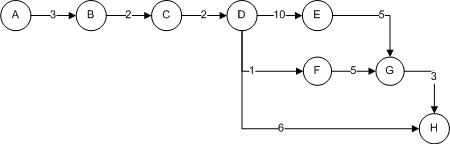
\includegraphics[width=130mm]{img/computation1.png}}}
\caption{Project Plan}
\label{pic:plan1}
\end{figure}
While usually the nodes are labelled with numbers, in this example the nodes are labelled with letters and the numbers are the duration of the activity. For example the activity AB has the duration 3.

\subsubsection{Forward Pass and Early Event Time}
As described at \ref{forwardPass} first the forward pass is made, determining the earliest finish time of the project and ES and EF of activities.

The project starts at event A, and therefore event A is labelled with 0. (\autoref{pic:plan_two})
\begin{figure}[h] 
\centerline{\fbox{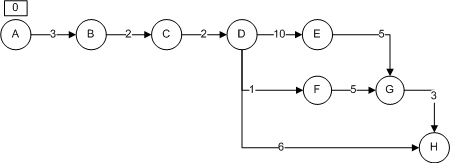
\includegraphics[width=130mm]{img/computation2.png}}}
\caption{Project Plan}
\label{pic:plan_two}
\end{figure}
After this it is easy to determine that event B can be reached within 3t, since there is only activity AB in between with duration 3. Event B is therefore labelled with 3.
To reach event C, two activities, namely AB and BC are necessary, with durations 3 and 2, therefore the earliest time event C can be reached is $3+2 = 5$. Event C is labelled with 5. (\autoref{pic:plan3})
\begin{figure}[h] 
\centerline{\fbox{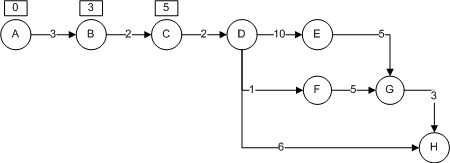
\includegraphics[width=130mm]{img/computation3.png}}}
\caption{Project Plan - Step 2}
\label{pic:plan3}
\end{figure}

Calculating the same for events D, E and F the diagram looks as shown in \autoref{fig:plan4}.
\begin{figure}[h] 
\centerline{\fbox{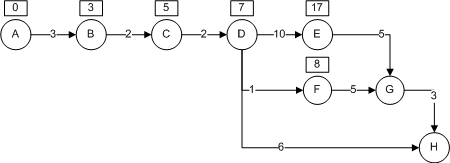
\includegraphics[width=130mm]{img/computation4.png}}}
\caption{Project Plan - Step 3}
\label{fig:plan4}
\end{figure}

Event G has two activities that lead into it, EG and FG, which both have the duration 5, but different time-labels at the previous events (17 and 8). The label of event G is calculated by $ max(label E + duration EG, label F + duration FG) = max(17+5, 8+5) = max(22,13) = 22 $. Doing the same for event H, the diagrams looks like \autoref{pic:plan5}.
\begin{figure}[h] 
\centerline{\fbox{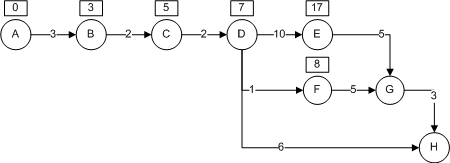
\includegraphics[width=130mm]{img/computation4.png}}}
\caption{Project Plan - Step 4}
\label{pic:plan5}
\end{figure}
\subsubsection{Backwards Pass and Late Event Time}
 Secondly the backward pass is done to determine the late event time and subsequently the LS and LF for each activity.
 The backward pass is basically the same as the forward pass, with the different that the last node is the starting node and the network is worked from the last node to the first node.

In this example, the start-node for the backwards pass is event H with late event time of 25. Event G for example is labelled with $ 25-3 = 22 $, and when 2 different activities lead into one event, it's late event time is the maximum of the predecessor-event (predecessor in the backward sense) minus the duration of the activity. This leads to \autoref{pic:plan6}
\begin{figure}[h] 
\centerline{\fbox{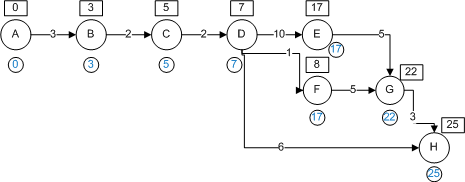
\includegraphics[width=130mm]{img/computation6.png}}}
\caption{final project plan}
\label{pic:plan6}
\end{figure}
The values added with the backward pass are in blue underneath each event.

\subsubsection{Activity Start and Finish Times}
From \autoref{pic:plan6} we can determine the ES, EF, LS, LF and TF of each activity. A typical activity looks as follows:
\begin{figure}[h] 
\centerline{\fbox{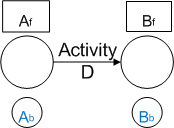
\includegraphics{img/activity_plan.png}}}
\caption{activity legend}
\label{pic:activity_plan}
\end{figure}
Each activity is bound by 2 events and has a Duration (D) and after completing the forward the ES can be calculated as follows:
\begin{equation}
ES = A_{f}
\end{equation}
If ES of an activity is know the EF can easily be determined by ES and B.
\begin{equation}
EF = ES + D
\end{equation}

If the backward pass was also completed successfully LF can be expressed as
\begin{equation}
LF = B_{b}
\end{equation}

After LF, the LS is obviously
\begin{equation}
LS = LF - D
\end{equation}

\subsubsection{Critical Path}

When applying the rules of \ref{determine_crit_path} the each activity is easily marked as critical or non-critical and the critical path becomes visible:
\begin{figure}[h] 
\centerline{\fbox{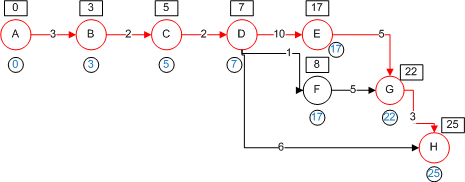
\includegraphics[width=130mm]{img/computation7.png}}}
\caption{final project plan - critical path}
\label{pic:plan7}
\end{figure}







\subsubsection{Checklist for Writing own CPM Spreadsheet / Software}
As a summary and when writing an own CPM Spreadsheet / Software, may it be in a spreadsheet-calculation program like Microsoft Excel or even designing an own software, the following rules/formulas must be defined:
\begin{itemize}
	\item The ES of the first activity is zero.
	\item The EF of any activity is $ES + D$.
	\item The ES of any activity is the latest of the EFs of all predecessors of that activity.
	\item The LF of the last activity in the project is equal to the EF of this activity. ($LF_{last} = EF_{last}$)
	\item The LS of any activity is $LF - D$
	\item The LF of any other activity except the last one is the earliest of all the LSs of all successors activities.
	\item The TF of any acitivity is equal to $LS - ES$ and also equal to $LF - EF$.
\end{itemize}
When following these rules, a basic CPM-algorithm can be implemented and the project-finish-date can be calculated after inputting a specific start date.













\section{Enhancements to the Basic System}
This section describes the most important enhancements of the basic CPM-System that have developed over time, and are found in the most recent software-CPM-programs. Some of these enhancements won't work with the basic formulas estabilished in \ref{formulas}, but still keep the basic functionality in tact.Others can be seen as just an extension of the basic system.

This list is in no way complete, since different programs implement different algorithms.

\subsection{Negative float}
When allowing a negative float in a CPM-System, one of the basic rules in the system "finish-to-start" is broken. This contraint is also called \textit{Finish not Later than (FNLT)}, which as seen by simple mathematics, if this FNLT-constraint is earlier than the standard LF, the Total Float will be a negative number.

With this FNLT constraint introduced there may arise some question to what is a critical activity now. For example if one activity has TF of minus two, does an activity with total float zero, which, by classic definition is a critical activity, still counts as critical? Furthermore, if the FNLT constraint is set to a later time then the calculated finish time, which value is used in further calculations? The answer to this last question depends on the program used, since there is no standard definition of this behaviour.

There also exists a SNLT (start not later than) contraint, which has the same problems as FNLT and should be used with caution as well.

\subsection{Actual Start and Finish Dates}

Another important enhancement of the standard CPM-system, is the ability to manually set start and finish dates. While it may be very convenient to just assign any single activity a specific value, this can lead to confusion depending on the exact algorithm used.

A typical problem is the "work out-of-sequence", with an activity started prior to completion of their predecessor activity.
There are many different ways in which software systems resolve this issue, among them the most popular:
\begin{itemize}
	\item Don't accept Inputs that may lead to this problem
	\item Write warning and generate output as good as possible
	\item Ignore this problem and use different algorithms to work toward the input dates.
\end{itemize}

\subsection{User Defined Codes \& Resources}

Sometimes it is very helpful for an end-user to add additional informations or resources to an activity, for example a supervising person responsible for an activity. While this is helpful as additional information, it should not be used to alter the network diagram in any way, or even assume that adding additional information is a replacement for other systems, like any resource-management-system. It can work in the small scale, but CPM is not made for managing to much additional information without compromising its original purpose.\\
An extra cost-field may be useful in determining if money can be saved, by looking at the non-critical activities and evaluating if more time can lead to less cost, but cannot replace a cost-management-system. 
\subsection{Calendars}

In the real word it is often the case that work can only be performed on work days (for example Monday till Friday) and even on these days only a specific amount of work hours are possible. If activities are scheduled in hours, using calendars is a very important concept.

On the other hand there are quite a few problems which need answering when using calendars:
\begin{itemize}
	\item \textbf{Float problem:} The TF depends on start and finish-date of an activity, but how is this calculated with weekends (non working days) in mind? For example if an activities ES is dated 1.1 and its LS 8.1, according to the formula $TF = LS - ES $ TF is 7 days. When considering a 5 day work calendar, the TF should only be 5 dys, since at least 1 weekend is in between. 
	\item \textbf{Multi-calendar Problem}: When working with multiple calendars at the same time, it may occur that an activity has 2 calendars assigned to it. For example an activity needs two limited Resources, each resource has a different calendar, it is not clear which calendar (and therefore work days etc.) to use. 
	\item \textbf{Displaying Problem}: A CPM diagram itself is pretty self-explanatory most of the time, but when using calendars it is not always clear if weekends or any holiday-calendars etc. are used by just looking at the diagram.
\end{itemize}

Still, taking aside these problems, using calendars is nowadays part of any modern CPM software and benefits the end-user significantly.

